\chapter{ตารางค่าพิกัดสีมาตรฐานสากลฉบับขยาย}
\label{app:color_tables}

\section{ตารางค่าพิกัดสีสารละลายดินครอบคลุม 4 ปริภูมิสี}

ตารางต่อไปนี้แสดงชุดพิกัดสีอ้างอิงเชิงมาตรวิทยา สำหรับการสอบเทียบระบบวิทัศน์ในระดับความเป็นกรดด่างตั้งแต่ 3.5 ถึง 9.0 พร้อมค่าพิกัดใน 4 ปริภูมิสี ได้แก่ sRGB, HSV, CIE $L^*a^*b^*$ และ YCbCr

\begin{table}[H]
\centering
\caption{ตารางพิกัดสีอ้างอิงสำหรับระดับความเป็นกรดด่างแบบละเอียด}
\label{tab:extended_ph_matrix}
\small
\begin{tabularx}{\textwidth}{c c c c c}
\toprule
\textbf{ระดับ pH} & \textbf{sRGB} & \textbf{HSV (องศา, \%, \%)} & \textbf{CIE $L^*a^*b^*$} & \textbf{YCbCr} \\
\midrule
3.5 & (183, 28, 28) & (0, 85, 72) & (37.1, 58.4, 42.1) & (73, 102, 206) \\
4.0 & (211, 47, 47) & (0, 78, 83) & (46.2, 63.8, 41.5) & (95, 101, 210) \\
4.5 & (230, 81, 0) & (21, 100, 90) & (53.4, 52.8, 64.9) & (118, 61, 207) \\
5.0 & (255, 152, 0) & (36, 100, 100) & (69.8, 32.1, 74.5) & (166, 34, 191) \\
5.5 & (255, 193, 7) & (45, 97, 100) & (80.1, 12.8, 81.3) & (194, 22, 171) \\
6.0 & (253, 216, 53) & (49, 79, 99) & (87.1, 0.4, 78.6) & (211, 38, 158) \\
6.5 & (139, 195, 74) & (88, 62, 76) & (73.5, -34.8, 52.4) & (172, 72, 104) \\
7.0 & (76, 175, 80) & (122, 57, 69) & (64.2, -45.1, 38.6) & (147, 90, 82) \\
7.5 & (0, 150, 136) & (174, 100, 59) & (56.4, -36.2, -1.2) & (121, 136, 42) \\
8.0 & (0, 188, 212) & (187, 100, 83) & (70.2, -31.4, -20.6) & (148, 164, 22) \\
8.5 & (63, 81, 181) & (231, 65, 71) & (38.8, 25.1, -55.8) & (88, 180, 110) \\
9.0 & (103, 58, 183) & (262, 68, 72) & (35.4, 45.2, -56.9) & (84, 183, 141) \\
\bottomrule
\end{tabularx}
\end{table}

\begin{figure}[H]
\centering
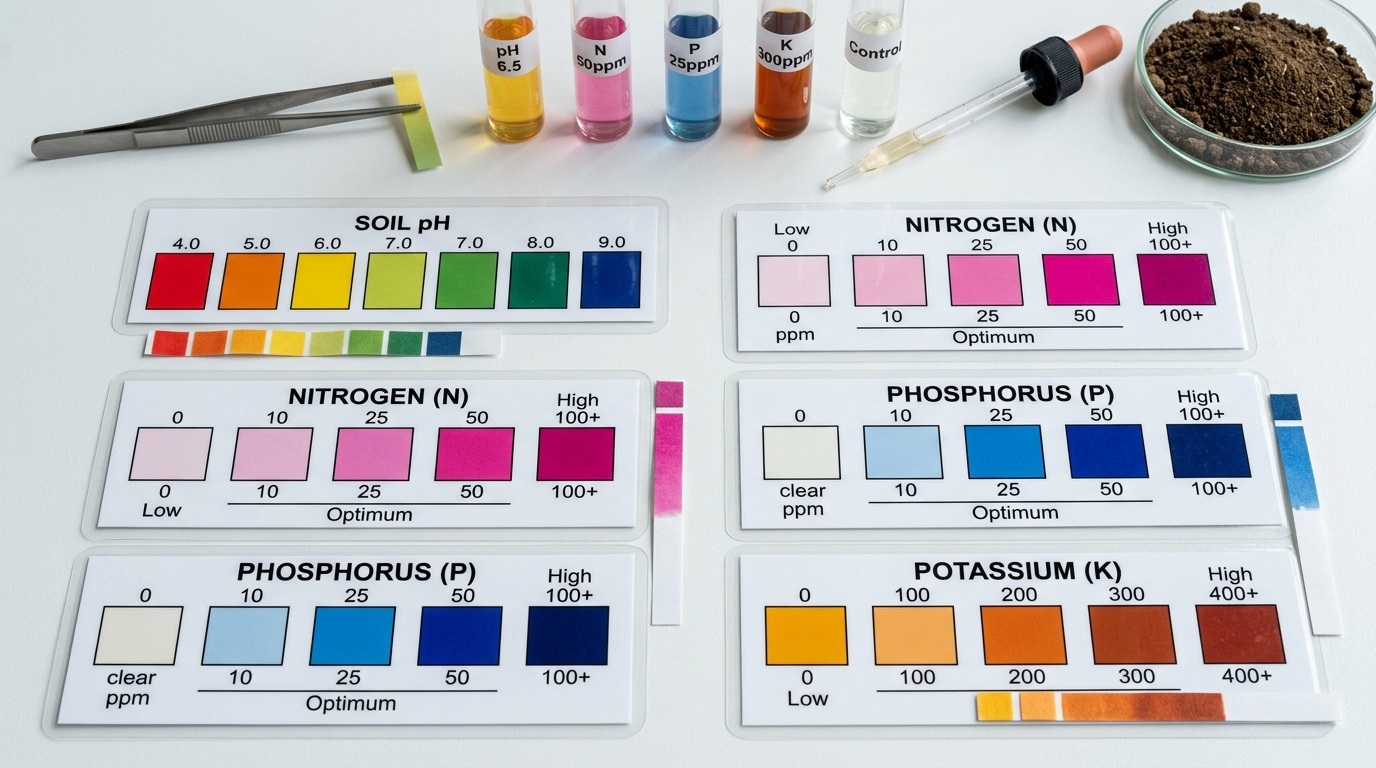
\includegraphics[width=0.88\textwidth]{figures/soil_npk_ph_chart.jpg}
\caption{แผนภูมิมาตรฐานเปรียบเทียบระดับสีทางเคมีสำหรับการประเมินค่าธาตุอาหาร N-P-K และความเป็นกรดด่าง}
\label{fig:soil_npk_ph_chart}
\end{figure}
